\documentclass[10pt,conference,letterpaper]{IEEEtran}

\usepackage{amsmath,amssymb}
\usepackage{graphicx}
\usepackage{booktabs}
\usepackage{tabularx}
\usepackage{array}
\usepackage{multirow}
\usepackage{algorithm}
\usepackage{algpseudocode}
\usepackage{xcolor}
\usepackage{microtype}
\usepackage{cite}
\usepackage{url}
\usepackage{stfloats}
\usepackage{placeins}

\usepackage{amsthm}
\newtheorem{lemma}{Lemma}
\newtheorem{theorem}{Theorem}
\providecommand{\FMtodo}[1]{\textbf{[AUTHOR INPUT: #1]}}

\newcommand{\method}{FedMATRIX-LoRA}
\newcommand{\best}[1]{\textbf{#1}}

\title{FedMATRIX-LoRA: Client-Aware Matrix-Level Adaptation for Resource-Constrained Federated Fine-Tuning}

\author{\IEEEauthorblockN{Anonymous Authors}}

\begin{document}
\maketitle

\begin{abstract}
Federated fine-tuning must reconcile heterogeneous client data with limited training resources. For low-rank adaptation (LoRA), the allocation problem concerns not only adapter capacity but also which target matrices each client should update. This paper presents FedMATRIX-LoRA, a client-aware matrix-level adaptation framework for resource-constrained federated fine-tuning. Each client evaluates candidate matrices using a local mini-batch at the current global adapter and constructs feasible configurations from the resulting importance scores. The server coordinates client participation and matrix configurations under a shared training budget and a round-latency objective. Selected adapters are trained locally and aggregated matrix-wise. This design couples data-dependent adaptation preferences with resource feasibility without changing the LoRA parameterization. Experiments on image classification, language understanding, and dialogue summarization show improvements over the evaluated baselines in task metrics and in resource efficiency under the adopted analytical client profiles.
\end{abstract}

\begin{IEEEkeywords}
Federated fine-tuning, low-rank adaptation, client-aware matrix selection, resource heterogeneity
\end{IEEEkeywords}

\section{Introduction}
% I1: Why the federated adaptation problem arises.
Foundation models provide reusable representations, but their adaptation often depends on data held by different institutions or devices. Federated learning enables these data holders to optimize a shared model without pooling their raw examples~\cite{mcmahan2017communication,kairouz2021advances}. The scale of pretrained models, however, makes full-parameter updates expensive for clients with limited memory, computation, and communication capacity. Low-rank adaptation (LoRA) reduces the trainable parameter set by representing weight updates through compact factors while keeping the pretrained backbone fixed~\cite{hu2022lora}. Federated LoRA thus makes collaborative adaptation more accessible, but it leaves an allocation question: which parts of the adapter should each client train with its available resources?

% I2: Explain the memory motivation without dismissing rank adaptation.
This question is not determined by adapter size alone. Training memory includes the frozen backbone, trainable parameters and their optimizer states, and intermediate activations required by backpropagation. Reducing rank shrinks the adapter-related state, but does not necessarily remove the backward computation needed to reach a trainable location. Fed-HeLLo identifies this distinction and reports limited total-memory savings from rank reduction when activations dominate~\cite{zhang2025fedhello}. Choosing trainable locations therefore complements rank adaptation: it changes both the parameters receiving updates and, under partial-adapter execution, the activation dependencies that must be retained. We study target selection at a fixed rank, separating this decision from the amount of capacity assigned within each selected adapter.

% I3: Introduce matrices before asking the reader to reason about selection.
A Transformer block contains several target projections, such as Query, Key, Value, and feed-forward transformations. Each can receive a distinct LoRA update, so a block-level allocation couples choices that can instead be made separately. The LoRA placement study and AdaLoRA's adaptive rank allocation already establish that adaptation value varies across matrices and layers~\cite{hu2022lora,fm_adalora2023}. These findings motivate treating the adapter subset as a decision variable rather than selecting a common location pattern and changing only its size. At a fixed rank, matrix-level selection allows a client to retain some projections within a block without assigning training capacity to every candidate projection in that block.

% I4: Explain importance and the role of the data distribution.
Selecting among these candidates requires an estimate of their value before committing a training budget. Importance scores provide such an estimate by measuring a parameter block's sensitivity to an adaptation objective. Gradient- and Fisher-based selection methods use information from the task loss to prioritize updates~\cite{fm_fish2021,zhang2025fedhello}. The data used for this assessment are consequential in federated learning: two clients can start from the same global adapter yet optimize different local objectives because their sample distributions differ. Accordingly, matrix importance should be understood as conditional on the model state and the data distribution, rather than as a fixed attribute of the pretrained architecture. This raises the question of whether a single importance vector adequately represents the adaptation priorities of heterogeneous clients.

% I5: Acknowledge existing client-aware work and state the specific focus.
Fed-HeLLo estimates layer importance on server-held proxy data and uses the resulting scores to guide client allocations~\cite{zhang2025fedhello}. A proxy distribution provides a shared reference, but may assign priorities different from those induced by an individual client's objective. Fed-pilot further incorporates local and globally aggregated importance information into memory-constrained LoRA allocation~\cite{fm_fedpilot2025}. Building on importance-guided adaptation, we investigate individual target-projection choices within each client and coordinate those choices under local memory and latency limits and a shared round budget. The resulting problem couples the source of importance information, the granularity of selection, and the feasibility of executing the selected updates.

% I6: Protocol only. No empirical outcome is available for this block yet.
A controlled motivating comparison is designed to distinguish differences in matrix priorities from their consequences for local adaptation. On CIFAR100 with ViT-base, it contrasts Local, which assigns each client its own scores; Local-Mean, which averages client scores into one shared vector; and Server-Proxy, which evaluates a separate server-held proxy set. The comparison spans IID data and Dirichlet partitions with concentration parameters $1.0$ and $0.1$. It holds the score formula, starting adapter, selected-matrix count, rank, local training length, and feasibility checks fixed within each comparison. Selection disagreement is measured separately from the reduction in held-out local validation loss. Local-Mean isolates the effect of sharing the same locally computed evidence, whereas Server-Proxy examines a distinct scoring-data source. The two planned panels in Fig.~\ref{fig:fm-motivation} connect these questions without equating different selections with better selections.
\FMtodo{Experiment P results are pending. Insert the verified selection-disagreement and paired validation-loss findings, with uncertainty, before drawing an empirical conclusion.}

\begin{figure}[!t]
  \centering
  \fbox{\parbox[c][1.2in][c]{.9\columnwidth}{\centering\FMtodo{Verified experiment P figure}}}
  \caption{Planned motivating comparison of scoring sources under data heterogeneity. (a) Jaccard distance between Local and Server-Proxy matrix selections. (b) Held-out local validation-loss reduction for Local, Local-Mean, and Server-Proxy at matched matrix counts, ranks, and training lengths. \FMtodo{Insert the verified P panels, seed set, aggregation unit, and uncertainty definition.}}
  \label{fig:fm-motivation}
\end{figure}

% I7: The two design requirements, not a list of solver achievements.
The methodological challenge has two parts. First, importance assessment must distinguish client-specific adaptation priorities at the current global model without requiring trial training of every candidate configuration. A low-cost gradient-based profile addresses this assessment problem. Second, those priorities must be translated into feasible allocations. A high-scoring subset can exceed a client's memory limit, and configurations that are feasible individually can jointly exceed the round budget or incur excessive synchronization latency. Thus, neither a shared importance ranking nor independent local selection alone specifies the desired training round. Client-conditioned assessment and resource-feasible coordination must be connected.

% I8: Explain the method through the two requirements.
We propose FedMATRIX-LoRA, a client-aware matrix-level adaptation framework for resource-constrained federated fine-tuning. During profiling refreshes, each client evaluates candidate LoRA factors on a local mini-batch at the current global adapter. The resulting scores define configuration priorities, while the resource model determines which configurations are feasible. Clients generate candidate configurations at different matrix-equivalent costs; the server coordinates participation and configuration choice under the shared budget and latency objective. Selected adapters are trained locally and aggregated matrix-wise to update a shared global adapter. In this design, local evidence determines preferred adaptation locations, and resource coordination determines which proposed updates can be executed together.

\begin{figure*}[t]
  \centering
  \resizebox{.84\textwidth}{!}{%
    \setlength{\unitlength}{1pt}%
    \begin{picture}(1159.92,472.08)
      \put(0,0){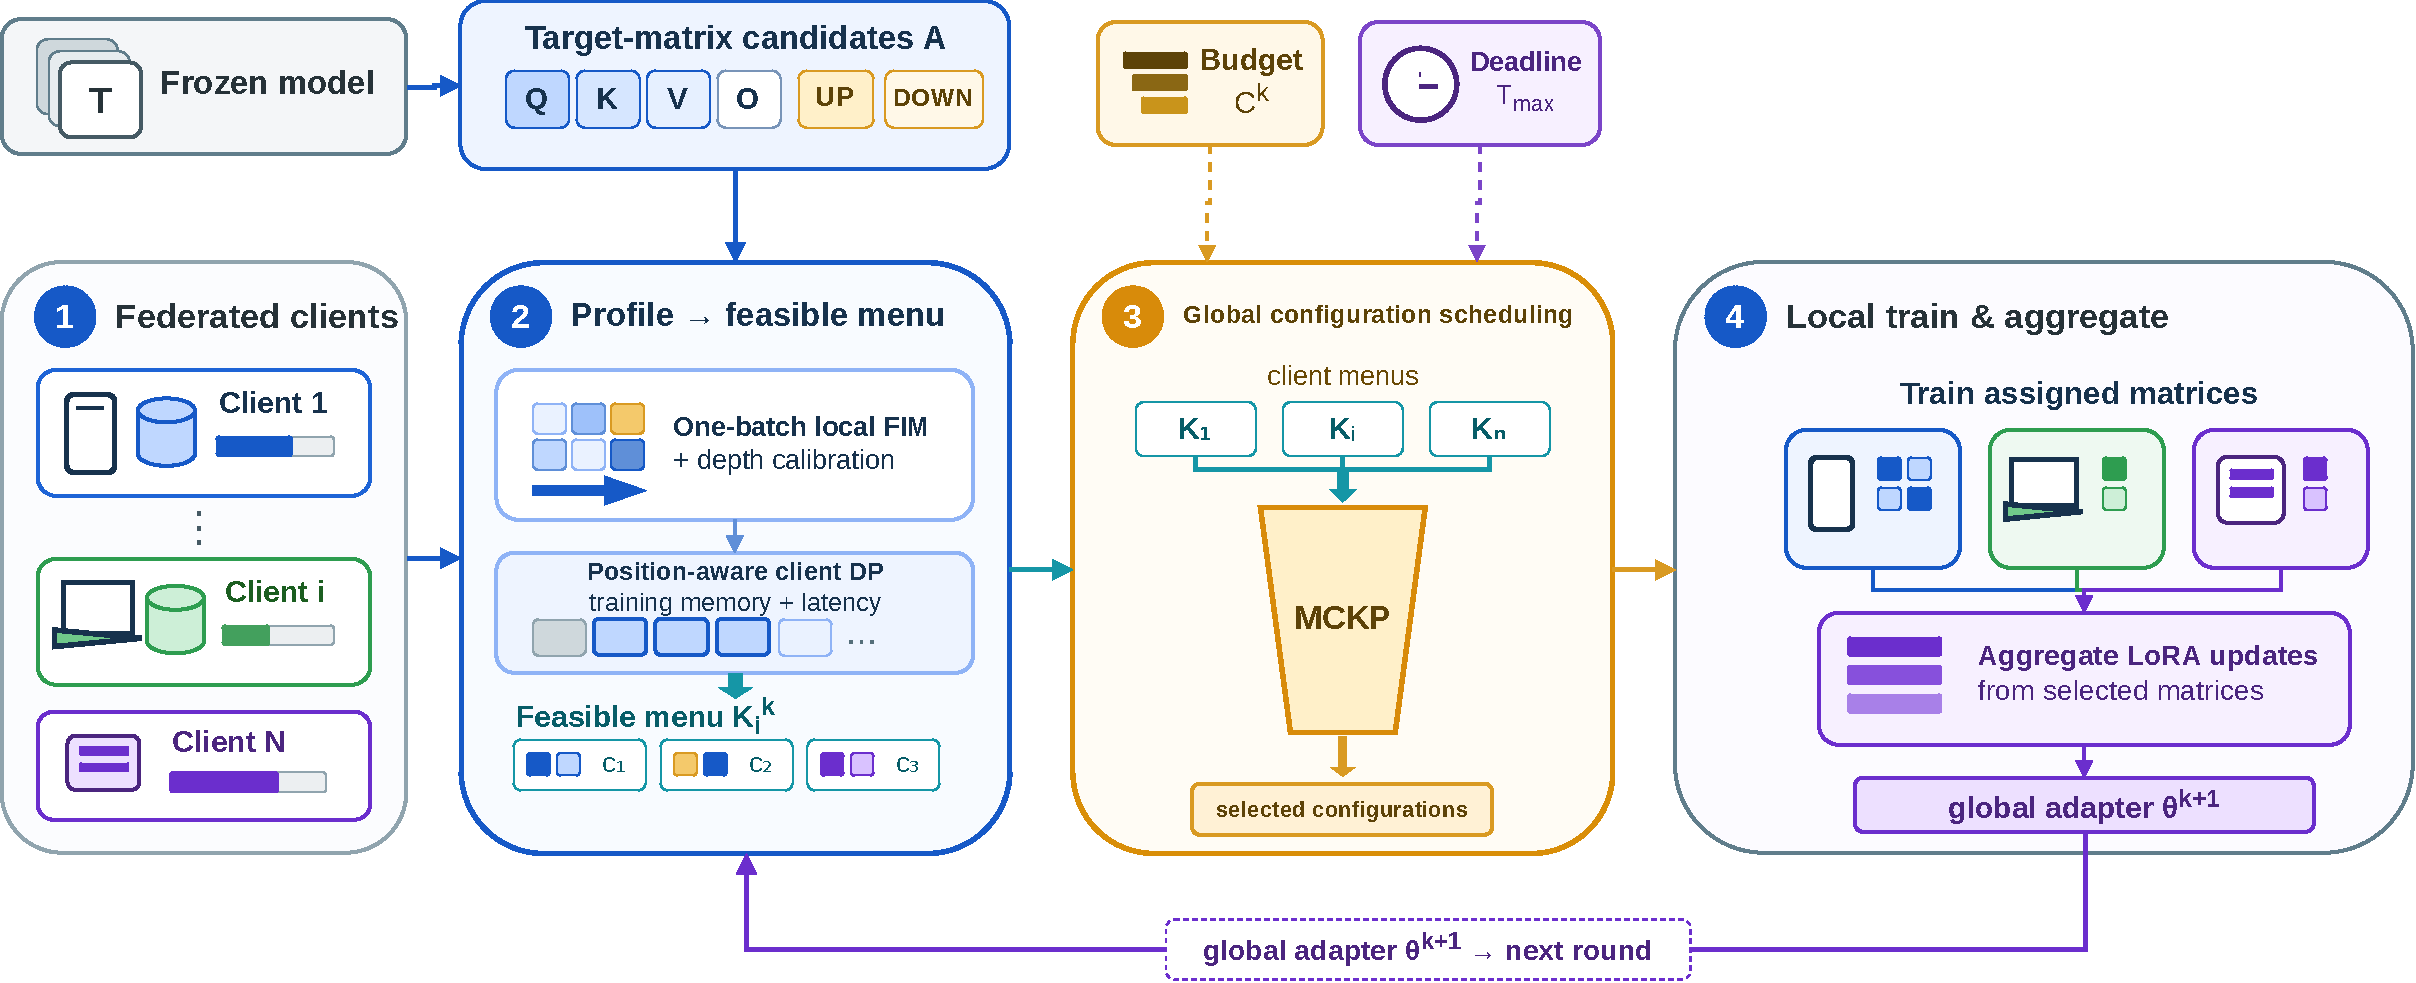
\includegraphics[width=1159.92pt]{figures/fig2_method_overview.pdf}}
      \put(321,242){\color{white}\rule{145pt}{35pt}}
      \put(323,261){\makebox(0,0)[l]{\color[HTML]{17324D}\fontsize{12}{13}\selectfont\sffamily\bfseries Local gradient-squared}}
      \put(323,247){\makebox(0,0)[l]{\color[HTML]{17324D}\fontsize{11}{12}\selectfont\sffamily profiling + depth calibration}}
      \put(618,158){\color[HTML]{FFF0C9}\rule{55pt}{37pt}}
      \put(645,183){\makebox(0,0){\color[HTML]{5D4308}\fontsize{9}{10}\selectfont\sffamily\bfseries Budget-}}
      \put(645,172){\makebox(0,0){\color[HTML]{5D4308}\fontsize{9}{10}\selectfont\sffamily\bfseries constrained}}
      \put(645,161){\makebox(0,0){\color[HTML]{5D4308}\fontsize{9}{10}\selectfont\sffamily\bfseries allocation}}
    \end{picture}%
  }
  \caption{\method{} workflow. Client-conditioned profiling scores target matrices; position-dependent training-memory and client-latency constraints shape feasible configurations; configuration-level global coordination selects among them under the round budget.}
  \label{fig:overview}
\end{figure*}

Our contributions are threefold:
\begin{itemize}
\item We formulate client-aware target-matrix selection for resource-constrained federated fine-tuning, making the trainable projection subset responsive to local data and device feasibility rather than specifying it solely through adapter capacity.
\item We develop FedMATRIX-LoRA, which connects local gradient-based profiling with feasible configuration generation and server coordination. The framework supports distinct projection choices within a Transformer block and across clients while maintaining a shared global adapter through matrix-wise aggregation.
\item We provide a conditional stationarity analysis that relates selective aggregation to effective-update bias and matrix coverage, and evaluate the complete framework on image classification, language understanding, and dialogue summarization under heterogeneous data and analytical resource profiles.
\end{itemize}

Section~\ref{Sec.relatedworks} positions the work relative to prior studies. Section~\ref{sec.model} presents the system model and problem formulation, and Section~\ref{Sec.alg} describes FedMATRIX-LoRA and its analysis. Section~\ref{Sec.evaluation} reports the evaluation, followed by the conclusion in Section~\ref{Sec.conclusion}.


\section{Related Work}\label{Sec.relatedworks}
\noindent\textbf{Parameter-efficient and selective adaptation.}
Parameter-efficient fine-tuning changes either the representation of an update or the subset of parameters that is trained. LoRA represents updates through low-rank factors attached to pretrained matrices, while QLoRA combines a quantized frozen backbone with trainable low-rank adapters~\cite{hu2022lora,dettmers2023qlora}. These mechanisms reduce different components of the adaptation footprint. Target selection introduces a further choice: an available adapter need not be trained on every client in every round. The distinction is useful in heterogeneous systems, where a common candidate architecture can admit different feasible trainable subsets.

Importance-aware methods provide a basis for making such choices. AdaLoRA assigns nonuniform rank budgets across weight matrices through importance-guided pruning of an SVD-style update parameterization~\cite{fm_adalora2023}. FISH constructs a sparse trainable-parameter mask from Fisher-based importance scores~\cite{fm_fish2021}. These methods demonstrate that uniform allocation is not the only way to organize a limited adaptation budget. FedMATRIX-LoRA applies importance-guided selection to a different decision: the fixed-rank target subset assigned to each federated client. Whereas within-matrix rank allocation controls adapter capacity, client-conditioned target selection determines the projections receiving that client's updates. Resource coordination then determines which client configurations can be executed together.

\noindent\textbf{Heterogeneous federated LoRA.}
HetLoRA supports heterogeneous client ranks and combines local rank self-pruning with server-side sparsity-weighted aggregation~\cite{cho2024hetlora}. FAH-QLoRA jointly considers quantization and LoRA rank in federated resource adaptation~\cite{gao2025fah}. These approaches establish the value of adapting capacity or numerical precision to client resources. As discussed by Fed-HeLLo, however, reducing rank primarily decreases optimizer-state memory in activation-dominated settings, motivating partial-layer training as a complementary allocation dimension~\cite{zhang2025fedhello}. LEGEND jointly configures tuning depth and rank distribution, explicitly connecting the location of trainable layers with resource use~\cite{liu2025legend}. Its combination of depth and rank illustrates that placement and capacity can jointly affect the resource--performance trade-off.

Fed-HeLLo further accounts for unequal layer importance through scores computed on server-held proxy data and geometric allocation strategies~\cite{zhang2025fedhello}. Its score-guided strategy converts a shared assessment into allocation probabilities; different clients can receive different masks even though the underlying importance evidence is shared. FedMATRIX-LoRA instead estimates importance on each client's data and exposes separate projection choices inside a block. This separates two aspects of heterogeneity: differences in client training capacity and differences in the data-dependent priorities used to allocate that capacity.

Fed-pilot is the closest importance-guided allocation counterpart. In its block-indexed formulation, local and cross-client, temporally aggregated information-gain scores guide memory-constrained LoRA allocation, and compensated aggregation addresses uneven updates~\cite{fm_fedpilot2025}. FedMATRIX-LoRA develops a different allocation formulation: independent target-projection indicators within blocks are coordinated across clients under memory limits, latency constraints, and a shared round budget. Local profiling is performed over the candidate target set at refresh rounds, and the resulting configurations are compared at the server. The formulation thereby connects within-block projection choices and client-specific importance with the feasibility of a jointly scheduled training round.

\noindent\textbf{Aggregation and resource coordination.}
Aggregation and allocation address related but distinct parts of federated adaptation. FedEx-LoRA treats the mismatch introduced by aggregating low-rank factors, while LoRA-FAIR studies aggregation and initialization refinement~\cite{singhal2025fedex,bian2025lorafair}. These directions concern how local updates are combined. Resource-aware methods such as Oort, FedBalancer, and PyramidFL address participant selection or training-work coordination under heterogeneous conditions~\cite{lai2021oort,shin2022fedbalancer,li2022pyramidfl}. In FedMATRIX-LoRA, the server decision also includes the trainable target subset assigned to a participating client. Feasible configurations therefore connect local adaptation preferences to the round-level allocation problem, rather than treating client participation and the internal trainable subset as unrelated decisions. The matrix-wise analysis characterizes the update pattern induced by this selective execution.

\section{System Model and Problem Formulation}\label{sec.model}

\subsection{System Model and Federated LoRA Preliminaries}
We consider a heterogeneous federated LoRA fine-tuning system consisting of one server and $N$ clients. Each client $i$ owns a private local dataset $\mathcal{D}_i$, an on-device training-memory capacity $M_i^{\max}$ (corresponding to the available GPU device memory in our implementation), an estimated communication bandwidth $B_i$, and heterogeneous computational resources. To preserve data privacy, all local datasets remain on their corresponding clients throughout the training process and are never uploaded to the server. The server initializes a pretrained backbone model $\Theta^0$, which remains frozen during federated fine-tuning, and maintains the global LoRA adapter parameters $\theta^k$ at communication round $k$.

Let $n_i=|\mathcal{D}_i|$ denote the number of local  training samples at client $i$. Federated LoRA fine-tuning aims to minimize the following global objective
\begin{equation}
F(\theta)=\frac{1}{N}\sum_{i=1}^{N}F_i(\theta),
\end{equation}
where
\begin{equation}
F_i(\theta)=
\frac{1}{n_i}
\sum_{z\in\mathcal{D}_i}
\ell(\Theta^0,\theta;z),
\label{eq:fl-objective}
\end{equation}
and $\ell(\cdot)$ denotes the task loss evaluated using the frozen backbone $\Theta^0$ and trainable LoRA parameters $\theta$.

For a target linear transformation $W_j\in\mathbb{R}^{d_{\mathrm{out}}\times d_{\mathrm{in}}}$, LoRA parameterizes its update as
\begin{equation}
\Delta W_j=B_jA_j,
\end{equation}
where $A_j\in\mathbb{R}^{r\times d_{\mathrm{in}}}$ and $B_j\in\mathbb{R}^{d_{\mathrm{out}}\times r}$ are low-rank matrices with rank $r\ll \min(d_{\mathrm{in}},d_{\mathrm{out}})$.

We treat the trainable adapter subset as a client-specific decision. A target matrix denotes a pretrained projection, such as Query, Key, or Value; selecting it means updating its associated LoRA factors, not the frozen pretrained matrix itself. The rank of every selected adapter is fixed to the same value, so configuration differences arise from target selection.

\subsection{Client-Aware Matrix-Level LoRA Allocation}
We formulate federated LoRA allocation at the target-matrix granularity.
Let
\begin{equation}
\mathcal{A}=\{W_1,W_2,\ldots,W_L\}
\end{equation}
denote the ordered set of LoRA-compatible target matrices extracted from the
backbone. These matrices include the Query, Key, Value, output, and feed-forward projection matrices in Transformer blocks. 

For client $i$ at communication round $k$, the matrix activation
decision is represented by the binary vector
\begin{eqnarray}
\mathbf m^k_i=[{m}_{i,1}^k,\cdots,{m}_{i,L}^k],
\end{eqnarray}
where
\begin{eqnarray}
&&{m}_{i,j}^k= \left\{
\begin{aligned}
&1,\mbox{if $W_j$ is activated for local training};\\
&0,\mbox{otherwise.}
\end{aligned}
\right.
\end{eqnarray}Each activation vector therefore specifies the subset of LoRA target matrices trained by client $i$ during communication round $k$.

Let $V_i^k(\mathbf m_i^k)$ denote the profiled utility of client $i$'s matrix configuration. It is computed from local data at the current global adapter and summarizes the estimated priority of the selected updates. We set $V_i^k(\mathbf 0)=0$. The profiling procedure is defined in Section~\ref{sec:fm-profiling}.

Layer-group allocation is recovered by constraining all candidate matrices in a Transformer block to share the same selection indicator.

\subsection{Resource Constraints and Problem Formulation}
The activation decision of LoRA target matrices determines the resource consumption of each participating client. We model the training cost, training-memory usage, and training latency separately.

First, let $c_i(\mathbf m^k_i)$ denote the normalized training cost associated with matrix configuration $\mathbf m^k_i$. We approximate this cost by the number of activated rank-8 matrices, $c_i(\mathbf m^k_i)=\sum_{j=1}^{L}m_{i,j}^k$. This standardized count is not a measurement of matrix-specific computation or memory, which can differ even at the same rank; memory is modeled separately below.


Training-memory consumption depends on both the number and positions of activated matrices. For any nonzero \(\mathbf m\), let
\(\mathcal{J}(\mathbf m)=\{j\mid m_j=1\}\) and \(j_{\min}(\mathbf m)=\min\mathcal{J}(\mathbf m)\).
Following the training-memory decomposition commonly adopted in partial-layer federated LoRA fine-tuning \cite{zhang2025fedhello}, we set \(M_i(\mathbf0)=M_i^{\mathrm{fixed}}\), while a nonzero configuration uses
\begin{equation}
M_i(\mathbf m)=M_i^{\mathrm{fixed}}+q_i(r)c_i(\mathbf m)+\sum_{j=j_{\min}(\mathbf m)}^{L}\mu_{i,j},
\label{eq:memory}
\end{equation}
where
$M_i^{\mathrm{fixed}}$
denotes the memory occupied by the frozen backbone and fixed runtime buffers,
$q_i(r)$ is the parameter-and-optimizer memory per activated rank-\(r\) LoRA matrix, and
$\mu_{i,j}$ is retained activation memory. The last term reflects the position-dependent memory characteristic of Transformer
fine-tuning: activating an earlier matrix requires retaining a longer backward propagation path and therefore consumes more activation memory. 

The latency of client $i$ consists of local computation and communication. Let $\gamma_i$ denote its computation coefficient, $\sigma_i$ the communication size per activated matrix, and $B_i$ its available bandwidth. Its latency is
\begin{equation}
\begin{aligned}
&&T_i^{\mathrm{comp}}(\mathbf m_i)=\gamma_i c_i(\mathbf m_i),\\
&&T_i^{\mathrm{comm}}(\mathbf m_i)=\frac{\sigma_i c_i(\mathbf m_i)}{B_i},\\
&&T_i(\mathbf m_i)=T_i^{\mathrm{comp}}(\mathbf m_i)+T_i^{\mathrm{comm}}(\mathbf m_i).
\end{aligned}
\label{eq:latency-model}
\end{equation}
The coefficients define an analytical resource profile; equal matrix-equivalent costs need not correspond to identical measured hardware costs.


At communication round $k$, the server jointly determines the participating clients and their matrix configurations under a shared resource budget. Let $S_k$ denote the set of candidate clients,
$z_i^k\in\{0,1\}$ indicate whether client $i$ participates in the current round,
$C^k$ denote the round-level training budget, and $\tau^k$ represent the latency of the current communication round. Let \(\ell_i^{\min}\) and \(\ell_i^{\max}\) bound the number of matrices activated by participating client \(i\), and let \(\lambda>0\) control the utility--latency trade-off.

\begin{align}
\max_{\{\mathbf m_i^k,z_i^k\},\tau^k}
\quad&
\sum_{i\in S_k}
V_i^k(\mathbf m_i^k)
-\lambda\tau^k
\label{eq:joint-objective}\\
\text{s.t.}\quad&
\sum_{i\in S_k}
c_i(\mathbf m_i^k)
\leq C^k,
\label{eq:joint-budget}\\
&
m_{i,j}^k\leq z_i^k,
\label{eq:participation}\\
&
\ell_i^{\min}z_i^k
\leq
\sum_{j=1}^{L}m_{i,j}^k
\leq
\ell_i^{\max}z_i^k,
\label{eq:bound}\\
&
M_i(\mathbf m_i^k)
\leq M_i^{\max},
\quad
\forall i:z_i^k=1,
\label{eq:joint-memory}\\
&
T_i(\mathbf m_i^k)
\leq
\tau^k
\leq
T_{\max},
\quad
\forall i:z_i^k=1 .
\label{eq:joint-latency}
\end{align}
The objective maximizes the aggregated client-conditioned adaptation utility while minimizing round latency. Equations~\eqref{eq:joint-budget}--\eqref{eq:joint-latency} impose the round-level matrix-equivalent budget, participation consistency, activated-matrix bounds, per-client training-memory limits, and the round deadline. In particular, Eqs.~\eqref{eq:participation} and \eqref{eq:bound} together ensure that an inactive client selects no matrix, whereas an active client selects between \(\ell_i^{\min}\) and \(\ell_i^{\max}\) matrices.


The formulation couples client-level feasibility with a shared round budget. We implement it by constructing feasible configurations locally and coordinating these configurations at the server.

\section{FedMATRIX-LoRA Design}\label{Sec.alg}
\subsection{Framework Overview}
FedMATRIX-LoRA links data-dependent matrix assessment to resource-feasible execution. As illustrated in Fig.~\ref{fig:overview}, clients profile candidate matrices at the current global adapter and construct configurations satisfying their local limits. The server coordinates these configurations under the round budget and latency objective. Clients then update the assigned adapters, and their results are aggregated matrix-wise. The scoring mechanism and the allocation procedure are described separately below.

\subsection{Client-Conditioned Matrix Profiling}\label{sec:fm-profiling}
\noindent\textbf{Client-conditioned assessment.}
Profiling supplies an importance estimate before a client's training configuration is selected. At a common global adapter, the local loss depends on the client's examples; its gradient therefore describes sensitivity to the parameters under that client's adaptation objective. A shared score vector summarizes a common reference objective, whereas separate local evaluations preserve differences among client objectives. We use this distinction to assign update priorities at the target-matrix level. The goal is to inform which LoRA factors a client should train, while the resource constraints in Section~\ref{sec:fm-allocation} determine which combinations can be executed.

\noindent\textbf{A single-pass gradient score.}
Gradient- and Fisher-based criteria have been used to select trainable parameters and LoRA layers~\cite{fm_fish2021,zhang2025fedhello}. We adopt a gradient-squared criterion because it can be evaluated for all candidate targets in one backward pass, without separately training each proposed configuration. During a refresh at round $k$, client $i$ attaches LoRA modules to the candidate projections, loads the current global adapter $\theta^k$, and evaluates the average loss on a local mini-batch $\mathcal B_i^k$. Let $\theta_j^k$ denote the LoRA factors associated with target matrix $j$. Its raw score is

\begin{equation}
 g_{i,j}^k=
 \sum_{p\in\theta_j^k}
 \left(
 \nabla_p
 \mathcal L_i(\theta^k;\mathcal B_i^k)
 \right)^2 .
 \label{eq:fim}
\end{equation}
The score measures the aggregate magnitude of the local batch-loss gradient over the adapter's trainable coordinates. Squaring makes contributions from different parameter coordinates nonnegative, and summation gives a block-level measure rather than an average sensitivity per parameter. For a fixed parameterization, a larger gradient norm indicates greater immediate loss sensitivity to a perturbation of that block, motivating its use as an update-priority signal. Because the calculation uses the gradient of a batch-averaged loss, we describe it as a Fisher-inspired proxy rather than an exact Fisher estimate. Its role is to rank candidate updates before local training, not to substitute for the observed task metric after training.

Both the local examples and $\theta^k$ enter the score. Consequently, clients may assign different priorities to the same target even when their models begin a round from the same global state. Re-evaluation at a later refresh also allows the priorities to change as the global adapter evolves. The single-pass design obtains a score for every candidate at a refresh, including candidates not selected for that client's preceding local update. This avoids restricting the next allocation decision to the client's previously active targets, without requiring trial optimization of the candidate configurations.

\noindent\textbf{Shared positional calibration.}
The data-dependent score is supplemented by a structural preference over candidate positions. Prior work on partial LoRA fine-tuning reports that deeper adaptation can provide favorable performance--resource trade-offs in the studied settings~\cite{liu2025legend}. We incorporate this observation through a multiplicative depth factor:
\begin{equation}
 \widetilde g_{i,j}^k=g_{i,j}^k(1+d_j)^{\rho},
 \label{eq:depth}
\end{equation}
Here $d_j=(j-1)/(L-1)$ is the normalized position in the ordered candidate set. For the evaluated configurations, $\rho=1+1.5\mathbb I_{\mathrm{pair}}+\eta$, where $\mathbb I_{\mathrm{pair}}$ indicates a sentence-pair task and $\eta=0,1,2$ denotes IID, ordinary non-IID, and severe non-IID settings, respectively. This is the specified calibration schedule; the local dependence remains in $g_{i,j}^{k}$.

The multiplier applies a common positional preference without replacing the client-specific evidence. It can change an individual client's ranking, but does not force clients with different raw scores to share a ranking or select the same matrices. This separates the source of importance information from the structural prior applied to it. The No-Depth comparison in Section~\ref{sec:fm-ablations} is designed to isolate the contribution of this calibration while retaining the local scoring and allocation procedures.

\noindent\textbf{Configuration utility and refresh.}
The server coordinates configurations proposed by different clients. We therefore use a common normalization scale rather than assigning a separate unit scale to each client's largest score:
\begin{equation}
G_{\max}^k=\max_{\substack{h\in S_k\\1\le j\le L}}\widetilde g_{h,j}^k,\qquad
 v_{i,j}^k=\frac{\widetilde g_{i,j}^k
 }{\max\{G_{\max}^k,\delta\}}\in[0,1],
 \label{eq:normalization}
\end{equation}
The positive constant $\delta$ prevents division by zero. Using the same divisor preserves the relative magnitudes of the calibrated scores across both clients and matrices, and sets the utility scale used in the server's utility--latency trade-off. For assignment $\mathbf m_i^k$, the configuration utility is $V_i^k(\mathbf m_i^k)=\sum_{j=1}^{L}m_{i,j}^{k}v_{i,j}^{k}$. Thus, local data determine the raw priorities, the depth factor supplies a structural preference, and the common scale makes those scores directly usable in the shared allocation objective. The sum is a configuration-selection proxy; it does not assume that the full training loss separates into independent matrix losses.

Scores are cached between designated refresh rounds and recomputed when the cache is unavailable or a refresh is due. Reuse avoids repeating the profiling pass at every allocation decision, while a refresh reconnects the score vector to the current adapter. Raw examples and profiling gradients remain local; coordination uses matrix scores and configuration summaries. The profiling sample count and refresh schedule are therefore part of the scoring protocol, rather than additional optimization variables. Section~\ref{sec:fm-score-study} specifies the controlled test of whether configuration scores rank short-term held-out loss reductions, and Section~\ref{sec:fm-ablations} specifies the end-to-end comparisons of scoring source, selection granularity, and calibration.

\subsection{Resource-Feasible Matrix Allocation}\label{sec:fm-allocation}
For a fixed round \(k\), superscripts are omitted from configuration attributes and scheduling variables when unambiguous. Each feasible configuration \(\kappa\) generated by client \(i\) is represented as
\[
\kappa=(V_{i\kappa},c_{i\kappa},T_{i\kappa},M_{i\kappa},\mathbf m_{i\kappa}),
\]
where \(V_{i\kappa}\), \(c_{i\kappa}\), \(T_{i\kappa}\), \(M_{i\kappa}\), and \(\mathbf m_{i\kappa}\) denote the profiled adaptation utility, normalized matrix-equivalent cost, estimated latency, estimated training-memory consumption, and binary target-matrix assignment, respectively. Each client uploads a compact configuration menu \(\mathcal K_i^k\).

\noindent\textbf{Local configurations.}
Under the adopted memory model, feasibility depends on the selected-matrix count and the earliest selected position through the retained-activation term. For each count $c$, the client therefore searches over feasible earliest positions and retains a configuration with the largest profiled utility. Let $Q_{i,e}^k(t)$ denote the maximum utility of selecting $t$ matrices from the suffix $\{e,\ldots,L\}$. Its recursion and the utility for configurations whose earliest selected position is $e$ are:
\(Q_{i,e}^k(0)=0\) and \(Q_{i,L+1}^k(t>0)=-\infty\).
\begin{equation}
 \begin{aligned}
 Q_{i,e}^k(t)&=\max\left\{Q_{i,e+1}^k(t),v_{i,e}^k+Q_{i,e+1}^k(t-1)\right\},\quad t\ge1,
 \\
 \Phi_{i,e}^k(c)&=v_{i,e}^k+Q_{i,e+1}^k(c-1).
 \end{aligned}
 \label{eq:client-dp}
\end{equation}

Only configurations satisfying the matrix-count, memory, and latency constraints are retained. Under the current count-based latency model, configurations with the same cost consume the same server budget and have the same latency; retaining the highest-utility feasible configuration at each cost therefore suffices for subsequent coordination.

\noindent\textbf{Server coordination.}
The server enumerates the distinct feasible latency thresholds $\tau\le T_{\max}$. For each threshold, it removes configurations exceeding $\tau$ and solves the remaining multiple-choice knapsack problem, choosing at most one configuration per client. With $H_i(w)$ denoting the largest utility attainable from the first $i$ client menus at budget $w$, the recursion is:

\begin{equation}
 H_i(w)=
 \max_{\kappa\in
 \mathcal K_i^k(\tau)\cup\{\varnothing\}:c_{i\kappa}\le w}
 \left\{
 H_{i-1}(w-c_{i\kappa})
 +
 V_{i\kappa}
 \right\},
 \label{eq:server-dp}
\end{equation}
Here $\mathcal K_i^k(\tau)$ is the menu after latency filtering, $\varnothing$ is the zero-utility inactive choice with zero cost, and $H_0(w)=0$.

The server selects the threshold and configuration assignment with the largest total utility minus $\lambda\tau$. This procedure optimizes the stated profiled objective; its role is to realize client-conditioned selection under the resource model. Algorithm~\ref{alg:fedmatrix} summarizes the complete training round.

\subsection{Local Training and Matrix-Wise Aggregation}

After determining the optimal configuration assignment, the server
dispatches the global adapter \(\theta^k\) together with the selected matrix
assignments to corresponding clients. Only selected LoRA parameters are updated locally. Task-specific trainable modules, if
required by the downstream task, are optimized jointly with the selected LoRA
parameters.

Since different clients may update different subsets of LoRA matrices, the
aggregation process is performed independently for each trainable matrix.
Let \(\mathcal U_j^k\) denote the clients returning updates for matrix \(j\), and let \(\theta_{i,j}^{k+1}\) be the corresponding locally updated LoRA parameters from client \(i\). The server performs matrix-wise client-uniform aggregation:

\begin{equation}
 \theta_j^{k+1}
 =
 \begin{cases}
 |\mathcal U_j^k|^{-1}
 \displaystyle\sum_{i\in \mathcal U_j^k}
 \theta_{i,j}^{k+1},
 &
 |\mathcal U_j^k|>0,
 \\[6pt]
 \theta_j^k,
 &
 |\mathcal U_j^k|=0 .
 \end{cases}
 \label{eq:aggregation}
\end{equation}

The updated global adapter is used to initialize the next round. Because the updating client set can differ across target matrices, the aggregation averages only the clients contributing to each matrix and preserves the previous value when no update is available.
\begin{algorithm}[t]
\caption{\method{} in communication round $k$}
\label{alg:fedmatrix}
\footnotesize
\begin{algorithmic}[1]
\Require
Global adapter \(\theta^k\),
candidate matrix set \(\mathcal A\),
candidate clients \(S_k\),
budget constraint \(C^k\),
latency bound \(T_{\max}\)
\Statex \hrulefill
\Statex \textit{Client-conditioned matrix profiling and allocation:}

\ForAll{\(i\in S_k\)}
    \If{profiling cache is unavailable or refresh is required}
        \State Insert LoRA modules on candidate matrices \(\mathcal A\)
        \State Compute matrix importance scores
        \(g_{i,j}^k\) using one local mini-batch
        \State Apply position-aware calibration
        to obtain \(\widetilde g_{i,j}^k\)
    \Else
        \State Reuse cached matrix importance scores
    \EndIf
    \State Normalize matrix utilities to obtain \(v_{i,j}^k\)
    \State Generate feasible configuration menu
    \(\mathcal K_i^k\) via suffix dynamic programming
\EndFor

\Statex \hrulefill
\Statex \textit{Resource-feasible server coordination:}

\State Initialize best objective value \(U^*\leftarrow -\infty\)
\ForAll{distinct feasible latency thresholds
\(\tau\leq T_{\max}\)}
    \State Remove configurations satisfying
    \(T_{i\kappa}>\tau\)
    \State Solve MCKP using dynamic programming
    under budget constraint \(C^k\)
    \State Compute objective value
    \(\sum_i\sum_{\kappa}x_{i\kappa}V_{i\kappa}
    -\lambda\tau\)
    \If{current objective \(>U^*\)}
        \State Update the best configuration assignment
    \EndIf
\EndFor

\Statex \hrulefill
\Statex \textit{Local training and matrix-wise aggregation:}
\State Dispatch selected matrix assignments and \(\theta^k\) to clients
\ForAll{selected clients}
    \State Train LoRA parameters only on assigned matrices
\EndFor
\State Perform matrix-wise aggregation to obtain
\(\theta^{k+1}\)
\State \Return updated global adapter \(\theta^{k+1}\)
\end{algorithmic}
\end{algorithm}

\subsection{Convergence of Matrix-Wise Aggregation}
\label{sec:fm-convergence}
We analyze the effective update induced by the matrix-wise aggregation rule. For this analysis, $\theta$ includes the LoRA parameters and any jointly trained shared task modules. Let $P^k$ project onto the parameter blocks selected for update in round $k$, as determined before local training. For a common positive round scale $\gamma$, define the actual aggregated direction by $v^k=(\theta^k-\theta^{k+1})/\gamma$. Conditioning on the current model, profiling information, and selected configuration, denoted by $\mathcal H_k$, write
\begin{align}
 b^k&=\mathbb E[v^k\mid\mathcal H_k]-P^k\nabla F(\theta^k),\\
 \xi^k&=v^k-\mathbb E[v^k\mid\mathcal H_k].
\end{align}
Thus $\mathbb E[\xi^k\mid\mathcal H_k]=0$, and the update is
\begin{equation}
 \theta^{k+1}=\theta^k-\gamma\bigl(P^k\nabla F(\theta^k)+b^k+\xi^k\bigr).
\end{equation}
The bias $b^k$ accounts for selective aggregation and the difference between local optimizer updates and the selected global gradient. This representation does not replace the experimental AdamW optimizer with SGD.

\noindent\textbf{Assumptions.}
Assume that $F$ is $\beta$-smooth on the relevant update segments and bounded below by $F_{\inf}$. Suppose the effective update errors satisfy
\begin{equation}
 \mathbb E\|b^k\|^2\le B_{\mathrm{upd}}^2,\qquad
 \mathbb E\|\xi^k\|^2\le S_{\mathrm{upd}}^2.
\end{equation}
We additionally assume effective matrix coverage: for some $0<\alpha_{\mathrm{cov}}\le1$ and $\varepsilon_{\mathrm{cov},k}\ge0$,
\begin{equation}
 \mathbb E\|P^k\nabla F(\theta^k)\|^2
 \ge\alpha_{\mathrm{cov}}\mathbb E\|\nabla F(\theta^k)\|^2
       -\varepsilon_{\mathrm{cov},k}.
\end{equation}
This condition quantifies the global gradient energy captured by the selected blocks.

\begin{theorem}[Expected stationarity]
\label{thm:fm-stationarity}
Under the stated assumptions, for $0<\gamma\le1/\beta$ and $K$ rounds,
\begin{align}
 \frac1K\sum_{k=0}^{K-1}\mathbb E\|\nabla F(\theta^k)\|^2
 \le{}&\frac{2D_0}{\alpha_{\mathrm{cov}}\gamma K}\\
 &+\frac{B_{\mathrm{upd}}^2+\beta\gamma S_{\mathrm{upd}}^2
              +\bar\varepsilon_{\mathrm{cov}}}{\alpha_{\mathrm{cov}}},\nonumber
\end{align}
where $D_0=F(\theta^0)-F_{\inf}$ for a fixed initialization and
$\bar\varepsilon_{\mathrm{cov}}=K^{-1}\sum_k\varepsilon_{\mathrm{cov},k}$.
\end{theorem}
For a fixed horizon, setting $\gamma=c/\sqrt K\le1/\beta$ yields an $O(K^{-1/2})$ optimization and noise term when the error bounds and coverage constant are uniform across the analyzed runs. The residual is governed by effective-update bias and uncovered gradient energy. The result characterizes average stationarity, rather than optimal test accuracy.

The contribution of client selection can be made explicit. Let $n_j=|\mathcal U_j|>0$, $g_{i,j}=\nabla_jF_i(\theta)$, $g_j=N^{-1}\sum_i g_{i,j}$, and $\zeta_j^2=N^{-1}\sum_i\|g_{i,j}-g_j\|^2$.
\begin{lemma}[Matrix-wise selection bias]
\label{lem:fm-selection-bias}
For any updating-client set $\mathcal U_j$,
\begin{equation}
 \left\|\frac1{n_j}\sum_{i\in\mathcal U_j}g_{i,j}-g_j\right\|^2
 \le\left(\frac N{n_j}-1\right)\zeta_j^2.
\end{equation}
\end{lemma}
The bound relates aggregation bias to participation and gradient heterogeneity at each target matrix. Proofs are provided in Appendix~\ref{app:fm-convergence}.



\section{Experiments}\label{Sec.evaluation}
In this section, we evaluate the effectiveness of the proposed \method{} through extensive simulations across diverse datasets and model settings. 

\subsection{Evaluation Setup}
We evaluate image classification on CIFAR100 \cite{krizhevsky2009cifar}, language understanding on MNLI, QNLI, QQP, and SST-2 from GLUE \cite{wang2019glue}, and dialogue summarization on SAMSum \cite{gliwa2019samsum}.

Table~\ref{tab:setup} gives the backbones, partitions, rounds, and rank-8 matrix-cost budgets; each round has ten clients. Classification uses equal random IID partitions or Dirichlet non-IID partitions with $\alpha=1.0$ or $0.1$. SAMSum uses contiguous length-sorted shards for severe skew and randomly assigned length-sorted shards for mild skew.

\begin{table*}[t]
\centering
\caption{Evaluation settings. Non-IID \(x\): Dirichlet \(\alpha=x\); Len-M/S: mild/severe length skew; slash-separated budgets follow partition order.}
\label{tab:setup}
\setlength{\tabcolsep}{4.0pt}
\begin{tabular}{@{}llllrrl@{}}
\toprule
Dataset & Task & Backbone & Partitions & Rounds & Cum. budget & Metric \\
\midrule
CIFAR100 & Image classification & ViT-base \cite{dosovitskiy2021vit} & IID, Non-IID 1.0/0.1 & 180 & 7,200/12,000 & Accuracy \\
MNLI & Language inference & DeBERTa-v3-large \cite{he2021deberta} & IID, Non-IID 1.0 & 50 & 9,500 & Accuracy \\
QNLI & Sentence-pair classification & RoBERTa-base \cite{liu2019roberta} & IID, Non-IID 1.0 & 80 & 4,800/7,200 & Accuracy \\
QQP & Paraphrase classification & DeBERTa-v3-large \cite{he2021deberta} & IID, Non-IID 1.0 & 50 & 9,500 & Accuracy \\
SST-2 & Sentiment classification & RoBERTa-base \cite{liu2019roberta} & IID, Non-IID 1.0 & 80 & 7,200 & Accuracy \\
SAMSum & Dialogue summarization & OPT-1.3B \cite{zhang2022opt} & IID, Len-M, Len-S & 40 & 10,000 & Rouge-L \\
\bottomrule
\end{tabular}
\end{table*}

\begin{figure*}[t]
  \centering
  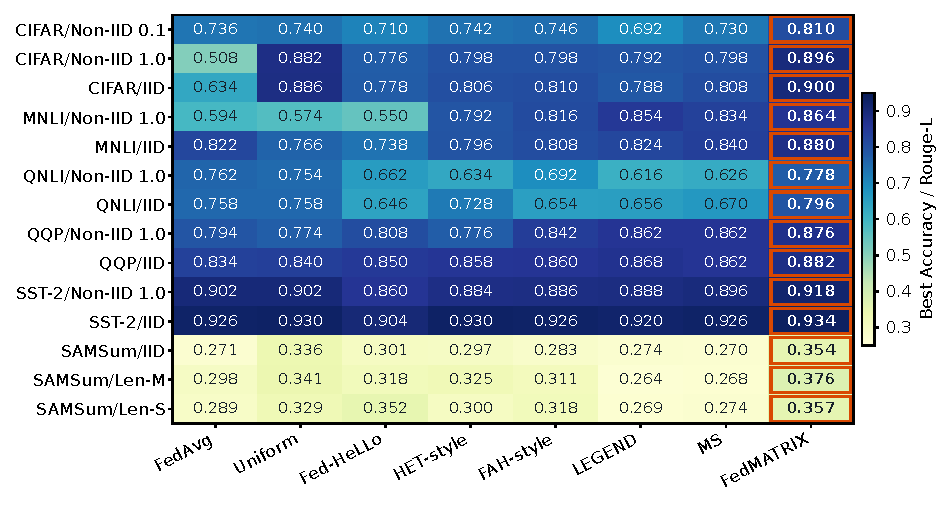
\includegraphics[width=.62\textwidth]{figures/fig3_main_results.pdf}
  \caption{Best task metric across 14 settings. Boxes mark row maxima; SAMSum uses Rouge-L and all other rows Accuracy.}
  \label{fig:matrix}
\end{figure*}

\begin{table}[t]
\centering
\caption{System and training profile.}
\label{tab:resource-profile}
\setlength{\tabcolsep}{3.6pt}
\begin{tabular}{@{}ll@{}}
\toprule
Control & Reported configuration \\
\midrule
Clients & 10 \\
Training-memory budget & 40/25/15 GB; ratio 6:3:1 \\
Compute factor & 0.8--2.0 s per rank-8 matrix-equivalent \\
Bandwidth & 5--50 MB/s \\
LoRA rank / profiling & 8 / one local mini-batch \\
Local training cap & one epoch, at most 50 mini-batch steps \\
Optimizer & AdamW \\
Batch size / learning rate & 1--32 / \(10^{-5}\)--\(10^{-4}\) \\
Default latency cap & 200 s per round \\
\bottomrule
\end{tabular}
\end{table}

Federated runs use NVIDIA A800-SXM4-80GB GPUs. Table~\ref{tab:resource-profile} gives the analytical client resource profiles and training settings. The main comparisons use seed 2024 with shared partitions and resource draws. The additional scoring and ablation studies report their seed sets and data splits separately. Cumulative training cost \(\overline C^K=\sum_{k=1}^{K}\sum_i c_i(\mathbf m_i^k)\) excludes profiling. Elapsed-time curves accumulate the analytical latency in Eq.~\eqref{eq:latency-model}, not end-to-end wall-clock time.

%Measured wall-clock times are reported separately in Section~V-E.




We report final and best Accuracy for classification and ROUGE-L for SAMSum, without averaging the two metrics.

We compare \method{} with representative baselines, including homogeneous LoRA training (FedAvg-LoRA) \cite{mcmahan2017communication,hu2022lora}, uniform matrix allocation (Uniform), layer-wise allocation (Fed-HeLLo) \cite{zhang2025fedhello}, layer-group heuristic allocation (MS), heterogeneous-rank allocation (LEGEND \cite{liu2025legend} and HETLoRA-style \cite{cho2024hetlora}), and joint quantization/rank allocation (FAH-QLoRA-style) \cite{gao2025fah}. These baselines represent different adaptation granularities and resource-allocation strategies, enabling a comprehensive comparison with our client-aware matrix scheduling. For a fair comparison, all methods use the same backbone models, data partitions, communication rounds, local training settings, and evaluation protocol.


\subsection{Task Performance and Resource Efficiency}
Fig.~\ref{fig:matrix} compares the best observed task metric across 14 evaluation settings. As shown in Fig.~\ref{fig:matrix}, \method{} consistently ranks first across all CIFAR100, GLUE, and SAMSum settings, covering both IID and heterogeneous data partitions. Compared with heterogeneous-rank and quantization-based baselines, \method{} also delivers substantially higher peak performance. For example, on MNLI IID, HETLoRA-style and FAH-QLoRA-style achieve $0.796$ and $0.808$, respectively, whereas \method{} reaches $0.880$. On CIFAR100 IID, the corresponding accuracies are $0.806$, $0.810$, and $0.900$, showing the performance of the complete framework under the reported evaluation protocol.

The budget--quality trajectories in Fig.~\ref{fig:budget-curves} characterize the performance obtained as the cumulative matrix-equivalent cost increases. Together with the matched-target comparison in Table~\ref{tab:time-to-quality}, they quantify the resource trade-off of the complete framework.

\begin{figure*}[!t]
  \centering
  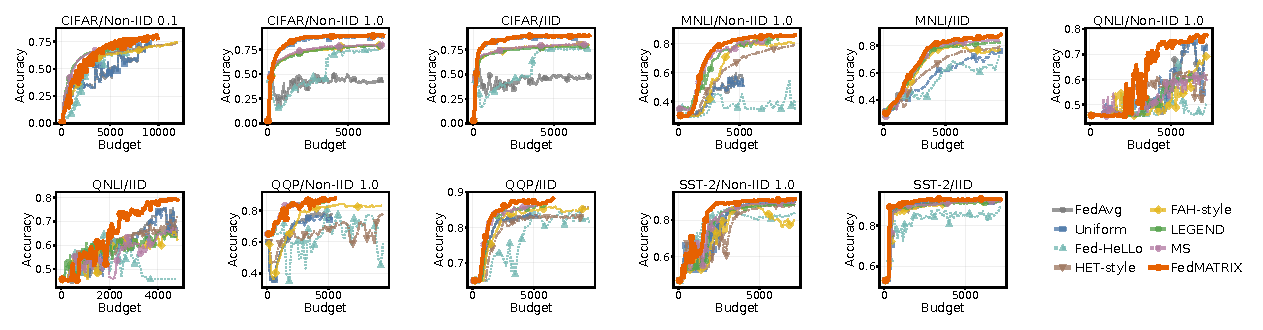
\includegraphics[width=.92\textwidth]{figures/fig4_budget_curves.pdf}
  \caption{Budget--quality trajectories for 11 classification scenarios; \method{} is emphasized.}
  \label{fig:budget-curves}
\end{figure*}

\begin{figure*}[!t]
  \centering
  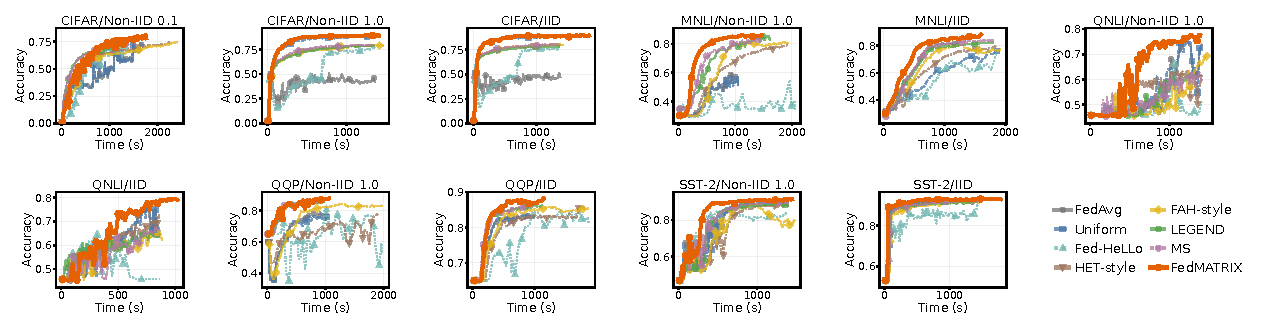
\includegraphics[width=.92\textwidth]{figures/fig5_time_curves.pdf}
  \caption{Modeled-time--quality trajectories for all 11 classification scenarios under the same analytical client profiles as Fig.~\ref{fig:budget-curves}.}
  \label{fig:time-curves}
\end{figure*}

Figure~\ref{fig:time-curves} reports the corresponding trajectories against cumulative modeled latency under the same analytical client profiles. The matched-target results in Table~\ref{tab:time-to-quality} summarize the modeled-time savings; these values are distinct from end-to-end measured runtime.

We additionally compare the resources required to reach the peak classification accuracy. Table~\ref{tab:time-to-quality} reports the cumulative-cost and modeled-time savings ($\Delta\overline C$ and $\Delta T$) of \method{} relative to the least-resource baseline reaching the same target. Across all $11$ classification scenarios, \method{} uses fewer resources, with median savings of $41.3\%$ in cumulative budget and $42.3\%$ in modeled elapsed time, demonstrating consistently higher resource efficiency across diverse workloads.

\begin{table}[!t]
\centering
\caption{Resources required to match each strongest baseline's peak Accuracy; positive savings favor \method{}.}
\label{tab:time-to-quality}
\setlength{\tabcolsep}{2.2pt}
\resizebox{\columnwidth}{!}{%
\begin{tabular}{@{}llrrr@{}}
\toprule
Scenario & Ref. & Target & $\Delta\overline C$ (\%) & $\Delta T$ (\%) \\
\midrule
CIFAR / Non-IID 0.1 & FAH-style & .746 & +53.9 & +59.4 \\
CIFAR / Non-IID 1.0 & Uniform & .882 & +42.9 & +42.4 \\
CIFAR / IID & Uniform & .886 & +54.4 & +48.3 \\
MNLI / Non-IID 1.0 & LEGEND & .854 & +5.6 & +27.7 \\
MNLI / IID & MS & .840 & +33.2 & +42.3 \\
QNLI / Non-IID 1.0 & FedAvg & .762 & +0.7 & +3.2 \\
QNLI / IID & FedAvg & .758 & +17.4 & +3.2 \\
QQP / Non-IID 1.0 & LEGEND & .862 & +14.9 & +21.7 \\
QQP / IID & LEGEND & .868 & +41.3 & +44.2 \\
SST-2 / Non-IID 1.0 & FedAvg & .902 & +44.4 & +45.2 \\
SST-2 / IID & HET-style & .930 & +47.8 & +38.5 \\
\bottomrule
\end{tabular}
}
\end{table}

\subsection{Scoring Reliability}\label{sec:fm-score-study}
We examine whether profiled configuration utility is associated with short-term local improvement. At each selected client and checkpoint, candidate configurations share the same rank, matrix-equivalent budget, and training length and include both score-guided and randomly generated feasible subsets. Each configuration is initialized from the same checkpoint, and improvement is measured as its own pre-training validation loss minus its post-training validation loss on held-out local examples. Spearman correlation is computed separately for each client--checkpoint pair before aggregation. Raw and depth-calibrated scores are evaluated against the same configuration outcomes.
\FMtodo{Insert verified A protocol: partition, checkpoint rounds, clients, configurations, steps, validation split, and seeds.}
\FMtodo{Insert A correlation table/figure and numeric findings; report the aggregation unit and uncertainty.}

\subsection{Ablation of Client-Aware Matrix Selection}\label{sec:fm-ablations}
We isolate the scoring source, selection granularity, and depth prior using controlled variants of the same training pipeline. Server-Proxy replaces client-specific scores with scores computed on a separate server-held proxy set. Layer-Level retains local assessment but ties together the candidate matrices within each Transformer block. No-Depth removes only the depth calibration. The full method serves as the reference. All variants share the predefined data splits, candidate-client protocol, optimizer settings, rank, resource limits, and training horizon; the selected participants and matrix subsets may differ as outcomes of the allocation procedure.
\FMtodo{Insert verified B metadata and mean/std results for final and best Accuracy, plus actual consumed matrix-equivalent budgets.}

Relative to Server-Proxy, Layer-Level, and No-Depth, the full method changes final Accuracy by \FMtodo{three signed percentage-point differences}, respectively, with the corresponding run-to-run variation reported in Table~\FMtodo{label}. The actual consumed budgets are \FMtodo{values}. These comparisons separate the effects of scoring source, matrix-level choice, and calibration within the evaluated setting.

\FloatBarrier
\section{Conclusion}\label{Sec.conclusion}
FedMATRIX-LoRA studies client-aware target-matrix selection for resource-constrained federated fine-tuning. Local profiling connects the current adapter to each client's data, while resource-feasible allocation coordinates the resulting preferences across clients. Matrix-wise aggregation supports the resulting heterogeneous update patterns. The reported experiments demonstrate the performance and resource trade-offs of the complete framework, and the conditional analysis relates its average stationarity to effective-update bias and matrix coverage.

\appendices
\section{Proofs for Matrix-Wise Aggregation}
\label{app:fm-convergence}
\begin{proof}[Proof of Theorem~\ref{thm:fm-stationarity}]
Condition on $\mathcal H_k$ and set $a=P^k\nabla F(\theta^k)$ and
$\bar v=\mathbb E[v^k\mid\mathcal H_k]=a+b^k$.
Because the update is supported on $P^k$, smoothness gives
\begin{align}
 \mathbb E[F(\theta^{k+1})\mid\mathcal H_k]
 \le{}&F(\theta^k)-\gamma\langle a,\bar v\rangle\\
 &+\frac{\beta\gamma^2}{2}
 \left(\|\bar v\|^2+\mathbb E[\|\xi^k\|^2\mid\mathcal H_k]\right).\nonumber
\end{align}
Use $2\langle a,\bar v\rangle=\|a\|^2+\|\bar v\|^2-\|b^k\|^2$ and
$\gamma\le1/\beta$ to discard the nonpositive term
$-\gamma(1-\beta\gamma)\|\bar v\|^2/2$. Taking total expectations yields
\begin{align}
 \mathbb E F(\theta^{k+1})\le{}&\mathbb E F(\theta^k)
 -\frac\gamma2\mathbb E\|P^k\nabla F(\theta^k)\|^2\\
 &+\frac\gamma2B_{\mathrm{upd}}^2
 +\frac{\beta\gamma^2}{2}S_{\mathrm{upd}}^2.\nonumber
\end{align}
Summing over $k$ telescopes the loss terms. The lower bound on $F$ gives
\begin{equation}
 \frac1K\sum_k\mathbb E\|P^k\nabla F(\theta^k)\|^2
 \le\frac{2D_0}{\gamma K}+B_{\mathrm{upd}}^2+\beta\gamma S_{\mathrm{upd}}^2.
\end{equation}
Apply the coverage condition and divide by $\alpha_{\mathrm{cov}}$.
\end{proof}

\begin{proof}[Proof of Lemma~\ref{lem:fm-selection-bias}]
Let $d_i=g_{i,j}-g_j$ and $w_i=\mathbf1\{i\in\mathcal U_j\}/n_j$.
Since $\sum_i d_i=0$, the selection bias equals $\sum_i(w_i-1/N)d_i$.
Cauchy--Schwarz gives
\begin{align}
 \left\|\sum_i(w_i-1/N)d_i\right\|^2
 &\le\sum_i(w_i-1/N)^2\sum_i\|d_i\|^2\\
 &=(1/n_j-1/N)N\zeta_j^2,
\end{align}
which is the claimed bound. For the full effective bias, define the remaining local-update discrepancy as $r=b-s$, with zero selection-bias blocks when no client updates a block. Then $\|b\|^2\le2\|s\|^2+2\|r\|^2$. The latter term includes local drift, optimizer effects, and any local-model mismatch; the selection lemma alone does not bound it.
\end{proof}


\clearpage
\begin{thebibliography}{99}
\bibitem{zhang2022opt}
S. Zhang \emph{et al.},
``OPT: Open pre-trained transformer language models,''
\emph{arXiv preprint arXiv:2205.01068}, 2022.

\bibitem{dosovitskiy2021vit}
A. Dosovitskiy \emph{et al.},
``An image is worth 16x16 words: Transformers for image recognition at scale,''
in \emph{Proceedings of the International Conference on Learning Representations (ICLR)}, 2021.

\bibitem{mcmahan2017communication}
B. McMahan, E. Moore, D. Ramage, S. Hampson, and B. A. y Arcas,
``Communication-efficient learning of deep networks from decentralized data,''
in \emph{Proceedings of the 20th International Conference on Artificial Intelligence and Statistics (AISTATS)}, 2017, pp. 1273--1282.

\bibitem{kairouz2021advances}
P. Kairouz \emph{et al.},
``Advances and open problems in federated learning,''
\emph{Foundations and Trends in Machine Learning}, vol. 14, nos. 1--2, pp. 1--210, 2021,
doi: 10.1561/2200000083.

\bibitem{hu2022lora}
E. J. Hu, Y. Shen, P. Wallis, Z. Allen-Zhu, Y. Li, S. Wang, L. Wang, and W. Chen,
``LoRA: Low-rank adaptation of large language models,''
in \emph{Proceedings of the International Conference on Learning Representations (ICLR)}, 2022.

\bibitem{cho2024hetlora}
Y. J. Cho, L. Liu, Z. Xu, A. Fahrezi, and G. Joshi,
``Heterogeneous LoRA for federated fine-tuning of on-device foundation models,''
in \emph{Proceedings of the 2024 Conference on Empirical Methods in Natural Language Processing}, 2024, pp. 12903--12913,
doi: 10.18653/v1/2024.emnlp-main.717.

\bibitem{gao2025fah}
Z. Gao, Z. Zhang, Y. Guo, and Y. Gong,
``Federated adaptive fine-tuning of large language models with heterogeneous quantization and LoRA,''
in \emph{Proceedings of IEEE Conference on Computer Communications (INFOCOM)}, 2025, pp. 1--10,
doi: 10.1109/INFOCOM55648.2025.11044641.

\bibitem{zhang2025fedhello}
Z. Zhang, P. Liu, J. Xu, and R. Hu,
``Fed-HeLLo: Efficient federated foundation model fine-tuning with heterogeneous LoRA allocation,''
\emph{IEEE Transactions on Neural Networks and Learning Systems}, vol. 36, no. 10, pp. 17556--17569, 2025,
doi: 10.1109/TNNLS.2025.3580495.

\bibitem{li2021moon}
Q. Li, B. He, and D. Song,
``Model-contrastive federated learning,''
in \emph{Proceedings of the IEEE/CVF Conference on Computer Vision and Pattern Recognition (CVPR)}, 2021, pp. 10713--10722,
doi: 10.1109/CVPR46437.2021.01057.

\bibitem{dettmers2023qlora}
T. Dettmers, A. Pagnoni, A. Holtzman, and L. Zettlemoyer,
``QLoRA: Efficient finetuning of quantized LLMs,''
in \emph{Advances in Neural Information Processing Systems}, vol. 36, 2023, pp. 10088--10115.

\bibitem{houlsby2019adapters}
N. Houlsby, A. Giurgiu, S. Jastrzebski, B. Morrone, Q. de Laroussilhe, A. Gesmundo, M. Attariyan, and S. Gelly,
``Parameter-efficient transfer learning for NLP,''
in \emph{Proceedings of the 36th International Conference on Machine Learning}, vol. 97, 2019, pp. 2790--2799.

\bibitem{li2021prefix}
X. L. Li and P. Liang,
``Prefix-tuning: Optimizing continuous prompts for generation,''
in \emph{Proceedings of the 59th Annual Meeting of the Association for Computational Linguistics and the 11th International Joint Conference on Natural Language Processing (Volume 1: Long Papers)}, 2021, pp. 4582--4597,
doi: 10.18653/v1/2021.acl-long.353.

\bibitem{zhang2023fedpetuning}
Z. Zhang, Y. Yang, Y. Dai, Q. Wang, Y. Yu, L. Qu, and Z. Xu,
``FedPETuning: When federated learning meets the parameter-efficient tuning methods of pre-trained language models,''
in \emph{Findings of the Association for Computational Linguistics: ACL 2023}, 2023, pp. 9963--9977,
doi: 10.18653/v1/2023.findings-acl.632.

\bibitem{chen2022fedtune}
J. Chen, W. Xu, S. Guo, J. Wang, J. Zhang, and H. Wang,
``FedTune: A deep dive into efficient federated fine-tuning with pre-trained transformers,''
\emph{arXiv preprint arXiv:2211.08025}, 2022.

\bibitem{che2023fedpeptao}
T. Che, J. Liu, Y. Zhou, J. Ren, J. Zhou, V. Sheng, H. Dai, and D. Dou,
``Federated learning of large language models with parameter-efficient prompt tuning and adaptive optimization,''
in \emph{Proceedings of the 2023 Conference on Empirical Methods in Natural Language Processing}, 2023, pp. 7871--7888,
doi: 10.18653/v1/2023.emnlp-main.488.

\bibitem{singhal2025fedex}
R. Singhal, K. Ponkshe, and P. Vepakomma,
``FedEx-LoRA: Exact aggregation for federated and efficient fine-tuning of large language models,''
in \emph{Proceedings of the 63rd Annual Meeting of the Association for Computational Linguistics (Volume 1: Long Papers)}, 2025, pp. 1316--1336,
doi: 10.18653/v1/2025.acl-long.67.

\bibitem{bian2025lorafair}
J. Bian, L. Wang, L. Zhang, and J. Xu,
``LoRA-FAIR: Federated LoRA fine-tuning with aggregation and initialization refinement,''
in \emph{Proceedings of the IEEE/CVF International Conference on Computer Vision (ICCV)}, 2025, pp. 3737--3746.

\bibitem{li2025telora}
Z. Li, B. Xu, X. Shu, J. Zhang, Y. Yao, G.-S. Xie, and J. Tang,
``Tensor-aggregated LoRA in federated fine-tuning,''
in \emph{Proceedings of the IEEE/CVF International Conference on Computer Vision (ICCV)}, 2025, pp. 1058--1067.

\bibitem{wang2026iflora}
H. Wang, X. Wang, Y. Li, J. Chen, J. Zhang, N. Yan, K. He, and W. Wang,
``Federated LoRA fine-tuning with pipelined error-mitigated aggregation and matrix-wise freezing,''
in \emph{Findings of the Association for Computational Linguistics: ACL 2026}, 2026, pp. 5749--5762,
doi: 10.18653/v1/2026.findings-acl.284.

\bibitem{bai2024flexlora}
J. Bai, D. Chen, B. Qian, L. Yao, and Y. Li,
``Federated fine-tuning of large language models under heterogeneous tasks and client resources,''
in \emph{Advances in Neural Information Processing Systems}, vol. 37, 2024, pp. 14457--14483,
doi: 10.52202/079017-0461.

\bibitem{koo2024loraa2}
J. Koo, M. Jang, and J. Ok,
``Towards robust and efficient federated low-rank adaptation with heterogeneous clients,''
in \emph{Proceedings of the 63rd Annual Meeting of the Association for Computational Linguistics (Volume 1: Long Papers)}, 2025, pp. 416--429,
doi: 10.18653/v1/2025.acl-long.19.

\bibitem{huang2026gmfl}
X. Huang, Y. Hu, Y.-J. Gong, and X. Zhang,
``GMFL: Efficient global masking for federated LLM fine-tuning,''
in \emph{Proceedings of the 64th Annual Meeting of the Association for Computational Linguistics (Volume 1: Long Papers)}, 2026, pp. 25293--25312,
doi: 10.18653/v1/2026.acl-long.1160.

\bibitem{ban2026fedalora}
H. Ban and K. Ji,
``Rethinking parameter sharing for LLM fine-tuning with multiple LoRAs,''
in \emph{Findings of the Association for Computational Linguistics: ACL 2026}, 2026, pp. 12843--12863,
doi: 10.18653/v1/2026.findings-acl.625.

\bibitem{diao2021heterofl}
E. Diao, J. Ding, and V. Tarokh,
``HeteroFL: Computation and communication efficient federated learning for heterogeneous clients,''
in \emph{Proceedings of the International Conference on Learning Representations (ICLR)}, 2021.

\bibitem{alam2022fedrolex}
S. Alam, L. Liu, M. Yan, and M. Zhang,
``FedRolex: Model-heterogeneous federated learning with rolling sub-model extraction,''
in \emph{Advances in Neural Information Processing Systems}, vol. 35, 2022, pp. 29677--29690.

\bibitem{lai2021oort}
F. Lai, X. Zhu, H. V. Madhyastha, and M. Chowdhury,
``Oort: Efficient federated learning via guided participant selection,''
in \emph{Proceedings of the 15th USENIX Symposium on Operating Systems Design and Implementation (OSDI)}, 2021, pp. 19--35.

\bibitem{shin2022fedbalancer}
J. Shin, Y. Li, Y. Liu, and S.-J. Lee,
``FedBalancer: Data and pace control for efficient federated learning on heterogeneous clients,''
in \emph{Proceedings of the 20th Annual International Conference on Mobile Systems, Applications and Services (MobiSys)}, 2022, pp. 436--449,
doi: 10.1145/3498361.3538917.

\bibitem{li2022pyramidfl}
C. Li, X. Zeng, M. Zhang, and Z. Cao,
``PyramidFL: A fine-grained client selection framework for efficient federated learning,''
in \emph{Proceedings of the 28th Annual International Conference on Mobile Computing and Networking (MobiCom)}, 2022, pp. 158--171,
doi: 10.1145/3495243.3517017.

\bibitem{kim2021autofl}
Y. G. Kim and C.-J. Wu,
``AutoFL: Enabling heterogeneity-aware energy efficient federated learning,''
in \emph{Proceedings of the 54th Annual IEEE/ACM International Symposium on Microarchitecture (MICRO)}, 2021, pp. 183--198,
doi: 10.1145/3466752.3480129.

\bibitem{luo2021costeffective}
B. Luo, X. Li, S. Wang, J. Huang, and L. Tassiulas,
``Cost-effective federated learning in mobile edge networks,''
\emph{IEEE Journal on Selected Areas in Communications}, vol. 39, no. 12, pp. 3606--3621, 2021,
doi: 10.1109/JSAC.2021.3118436.

\bibitem{kirkpatrick2017ewc}
J. Kirkpatrick \emph{et al.},
``Overcoming catastrophic forgetting in neural networks,''
\emph{Proceedings of the National Academy of Sciences of the United States of America}, vol. 114, no. 13, pp. 3521--3526, 2017,
doi: 10.1073/pnas.1611835114.

\bibitem{liu2025legend}
J. Liu, Y. Liao, H. Xu, Y. Xu, J. Liu, and C. Qian,
``Adaptive parameter-efficient federated fine-tuning on heterogeneous devices,''
\emph{IEEE Transactions on Mobile Computing}, vol. 24, no. 11, pp. 12533--12549, 2025,
doi: 10.1109/TMC.2025.3586644.

\bibitem{krizhevsky2009cifar}
A. Krizhevsky,
``Learning multiple layers of features from tiny images,''
Department of Computer Science, University of Toronto, Toronto, ON, Canada, Technical Report, 2009.

\bibitem{wang2019glue}
A. Wang, A. Singh, J. Michael, F. Hill, O. Levy, and S. R. Bowman,
``GLUE: A multi-task benchmark and analysis platform for natural language understanding,''
in \emph{Proceedings of the International Conference on Learning Representations (ICLR)}, 2019.

\bibitem{gliwa2019samsum}
B. Gliwa, I. Mochol, M. Biesek, and A. Wawer,
``SAMSum corpus: A human-annotated dialogue dataset for abstractive summarization,''
in \emph{Proceedings of the 2nd Workshop on New Frontiers in Summarization}, 2019, pp. 70--79,
doi: 10.18653/v1/D19-5409.

\bibitem{he2021deberta}
P. He, X. Liu, J. Gao, and W. Chen,
``DeBERTa: Decoding-enhanced BERT with disentangled attention,''
in \emph{Proceedings of the International Conference on Learning Representations (ICLR)}, 2021.

\bibitem{liu2019roberta}
Y. Liu \emph{et al.},
``RoBERTa: A robustly optimized BERT pretraining approach,''
\emph{arXiv preprint arXiv:1907.11692}, 2019.

\bibitem{fm_adalora2023}
Q. Zhang, M. Chen, A. Bukharin, N. Karampatziakis, P. He, Y. Cheng, W. Chen, and T. Zhao,
``AdaLoRA: Adaptive budget allocation for parameter-efficient fine-tuning,''
\emph{arXiv preprint arXiv:2303.10512}, version 2, 2023.

\bibitem{fm_fish2021}
Y.-L. Sung, V. Nair, and C. Raffel,
``Training neural networks with fixed sparse masks,''
in \emph{Advances in Neural Information Processing Systems}, vol. 34, 2021.

\bibitem{fm_fedpilot2025}
Z. Zhang, R. Hu, P. Liu, and J. Xu,
``Fed-pilot: Optimizing LoRA allocation for efficient federated fine-tuning with heterogeneous clients,''
\emph{arXiv preprint arXiv:2410.10200}, version 2, 2025.
\end{thebibliography}

\end{document}
